% ==================================================
% FSE demo paper
%    4 pages in the ACM proceedings format, including all text, references and figures.
%
%   Accompanied by:
%     1. a link to screencast of 5 to 10 minutes
%     2. a link to the website for this tool
%     3. information on tool availability and maturity 
%
%   Paper    submission : November 20, 2017
%   Author   notification : January 22, 2018
%   Camera-ready deadline : February 12, 2018
% ==================================================
\documentclass[sigconf]{acmart}
%\pdfpagewidth=8.5in
%\pdfpageheight=11in
% !TEX root = ./1critics.tex
% -----------------------------------------------------------------
% package
% -----------------------------------------------------------------
\usepackage{color}
\usepackage{xcolor}
\usepackage{xspace}
\usepackage[utf8]{inputenc}
\usepackage{algpseudocode}
%\usepackage[noend]{algorithmic}
\usepackage{amssymb}
\usepackage{pifont}
\usepackage{alltt}
\usepackage{framed,color}
\usepackage{multirow}
\usepackage{enumerate}
%\usepackage{enumitem} % for better lists
\usepackage{colortbl} % for table highlighting
\makeatletter
\newif\if@restonecol
\makeatother
\let\algorithm\relax
\let\endalgorithm\relax
\usepackage[ruled,vlined,noend]{algorithm2e}
%\usepackage[algo2e]{algorithm2e} 
\usepackage{stmaryrd} %for arrows
\usepackage{listings} %for code snippets
\usepackage{url}
\usepackage{pgfplots}
\usepackage{tikz}
\usepackage{balance}
\usepackage[listings]{tcolorbox}
\usepackage{graphicx}
\usepackage{caption}
\usepackage{subcaption}
\usepackage{qtree}
\usepackage{booktabs}
\makeatletter  
 \let\@copyrightspace\relax  
\makeatother  
\usepackage{soulutf8}

% -----------------------------------------------------------------
% color
% -----------------------------------------------------------------
\definecolor{darkBlue}{rgb}{0.000000,0.000000,0.545098}
\definecolor{darkGreen}{rgb}{0.000000,0.392157,0.000000}
\definecolor{DarkGray}{gray}{0.4}
\definecolor{javared}{rgb}{0.6,0,0} % for strings
\definecolor{javagreen}{rgb}{0.25,0.5,0.35} % comments
\definecolor{javapurple}{rgb}{0.5,0,0.35} % keywords
\definecolor{javadocblue}{rgb}{0.25,0.35,0.75} % javadoc
\definecolor{lightgray}{gray}{0.8}
\definecolor{lightblue}{rgb}{0.63, 0.79, 0.95}
\definecolor{shadecolor}{RGB}{150,150,150}
\definecolor{blueA}{RGB}{204,229,255}
\definecolor{redA}{RGB}{112,0, 0}
% -----------------------------------------------------------------
% abbreviations
% -----------------------------------------------------------------
\newcommand{\jinn}{Jinn\xspace}
\newcommand{\hidden}[1]{}
\newcommand{\xtc}{{\small\textsf{xtc}}}
\newcommand{\rats}{\textit{Rats!}}
\newcommand{\typical}{{\small\textsf{Typical}}}
\newcommand{\gctk}{GCTk\xspace}
\newcommand{\mmtk}{MMTk\xspace}
\newcommand{\jikes}{Jikes RVM\xspace}
\newcommand{\jikesrvm}{\jikes\xspace}
\newcommand{\jala}{Jalape\~{n}o\xspace}
\newcommand{\jalapeno}{Jalape\~{n}o\xspace}
\newcommand{\specjvm}{SPEC JVM\xspace}
\newcommand{\jess}{\textsf{\_202\_jess}\xspace}
\newcommand{\raytrace}{\textsf{\_205\_raytrace}\xspace}
\newcommand{\db}{\textsf{\_209\_db}\xspace}
\newcommand{\javac}{\textsf{\_213\_javac}\xspace}
\newcommand{\jack}{\textsf{\_228\_jack}\xspace}
\newcommand{\compress}{\textsf{\_201\_compress}\xspace}
\newcommand{\mpegaudio}{\textsf{\_222\_mpegaudio}\xspace}
\newcommand{\mtrt}{\textsf{\_227\_mtrt}\xspace}
\newcommand{\jbb}{\textsf{pseudojbb}\xspace}
\newcommand{\dacapo}{\textsf{DaCapo}\xspace}
\newcommand{\dacapover}{\textsf{DaCapo b.050224}\xspace}
\newcommand{\antlr}{\textsf{antlr}\xspace}
\newcommand{\bloat}{\textsf{bloat}\xspace}
\newcommand{\chart}{\textsf{chart}\xspace}
\newcommand{\eclipse}{\textsf{eclipse}\xspace}
\newcommand{\fop}{\textsf{fop}\xspace}
\newcommand{\hsqldb}{\textsf{hsqldb}\xspace}
\newcommand{\jython}{\textsf{jython}\xspace}
\newcommand{\luindex}{\textsf{luindex}\xspace}
\newcommand{\lusearch}{\textsf{lusearch}\xspace}
\newcommand{\pmd}{\textsf{pmd}\xspace}
\newcommand{\ps}{\textsf{ps}\xspace}
\newcommand{\xalan}{\textsf{xalan}\xspace}
\newcommand{\psfun}{\textsf{ps-fun}\xspace}
\newcommand{\ipsixql}{\textsf{ipsixql}\xspace}
\newcommand{\Ginseng}{{\sc Ginseng}\xspace}
\newcommand{\fixme} [1] {\textcolor{red}{{\it FIXME}: #1}}
%\newcommand{\fixme} [1] {}
\newcommand{\factfont}[1]{\scriptsize{{{#1}}}\normalsize}
\newcommand{\codefont}[1]{\footnotesize{\texttt{#1}}\normalsize}
\newcommand{\sydit}{\small \sc Sydit}
\newcommand{\reffinder}{\small \sc RefFinder}
\newcommand{\faulttracer}{\small \sc FaultTracer}
\newcommand{\iberry}{\small \sc Iberry}
\newcommand{\abs}[1]{\lvert#1\rvert}
\newcommand{\lase}{{\small {\sc Lase}}}
\newcommand{\genprog}{\small \sc GenProg}
\newcommand{\lsdiff}{\small \sc LSDiff}
\newcommand{\tool}{{\small{\sc{Critics}}}}
\newcommand{\collaborator}{{\small{\sc{Collaborator}}}}
\newcommand{\cTrans}{{\small{\sc{Grafter}}}}
\newcommand{\grafter}{{\small{\sc{Grafter}}}}
\newcommand{\deckard}{{\small {\sc Deckard}}}
\newcommand{\major}{{\small {\sc Major}}}
\newcommand{\uscalpel}{{\small {\sc $\mu$SCALPEL}}}
\newcommand*{\MyIndent}{\hspace*{0.3cm}}%


% -----------------------------------------------------------------
% misc
% -----------------------------------------------------------------
\newcommand{\codeTrans}{\textcolor{red}}
\newcommand{\dataTrans}{\textcolor{blue}}
\newcommand{\addCode}{\textcolor{black}}
\newcommand{\ax}{\textcolor{blue}{+}}
\newcommand{\delCode}{\textcolor{black}}
\newcommand{\dx}{\textcolor{red}{-}}
\newcommand{\susCode}{\textcolor{javagreen}}
\newcommand{\undoCode}{\textcolor{javagreen}{*}}
\newcommand{\myhref}[2]{\texttt{\scriptsize{\href{#1}{#2}}}}
\newcommand{\fix}[2]{\textbf{#1 asks:~\emph{ #2}}}
\newcommand{\pagemark}[1]{\textcolor{blue}{PAGE: {#1}}}
\newcommand{\todo}[1]{{\textcolor{blue}{{\bf TODO}: {#1}}}}
%\newcommand{\todo}[1]{}
\newcommand{\diffa}[1]{{\textcolor{red}{{#1}}}}
\newcommand{\diffb}[1]{{\textcolor{blue}{{#1}}}}
%\newcommand{\old}[1]{{\textcolor{red}{{}{}}}}
%\newcommand{\old}[1]{{\textcolor{red}{{\bf Old}: {#1}}}}
\newcommand{\oo}[1]{{\scriptsize{\textcolor{red}{{\bf*} {#1}}}}}
\newcommand{\ignore}[1]{}
\newcommand{\mccenter}[1]{\multicolumn{1}{c|}{#1}}
\newcommand{\m}[1]{\textcolor{blue}{#1}}
\newcommand{\selectbox}[1]{\par\colorbox{blueA}
{\parbox{\dimexpr\textwidth-17\fboxsep\relax}{#1}}}
\newcommand{\hilight}[1]{\colorbox{blueA}{#1}}
\newcommand{\hilightR}[1]{\colorbox{red}{\textcolor{yellow}{#1}}}
\newcommand{\fn}[1]{\footnote{\scriptsize{#1}}}
% \newcommand{\textsubscript}[1]{$_{\text{#1}}$}
\newcommand{\ttt}[1]{\tt\small{#1}}
\newcommand{\tttt}[1]{\tt\scriptsize{#1}}
\newcommand{\new}[1]{{\textcolor{blue}{{#1}}}}
\newcommand{\old}[1]{\textcolor{red}{\st{#1}}}

% -----------------------------------------------------------------
% indent dense
% -----------------------------------------------------------------
\def\denseitems 
{
  \itemsep1pt plus1pt minus1pt
  \parsep0pt plus0pt
  \parskip0pt\topsep0pt
}
% -----------------------------------------------------------------
% 
% -----------------------------------------------------------------
\chardef\oc=`\{
\chardef\cc=`\}
\chardef\us=`\_
\def\Note#1{\emph{\textbf{\small $<$#1$>$}}}
% -----------------------------------------------------------------
% 
% -----------------------------------------------------------------
\newcommand{\cmark}{\ding{51}}%
\newcommand{\xmark}{\ding{55}}%
\newcommand{\xxx}{\ding{53}}
\newcommand*{\smalltt}[1]{\texttt{\small{}#1}}
% ===============================================
% MyJavaStyle
% ===============================================
\lstdefinestyle{MyJavaStyle} {
  language=Java,
  frame=lines,
  xleftmargin=15pt, 
  stepnumber=1, 
  numbers=left, 
  numbersep=5pt,
  numberstyle=\tiny\color[gray]{0.777}, 
  belowcaptionskip=\bigskipamount,
  captionpos=b, 
  escapeinside={*'}{'*},
  tabsize=5,
  emphstyle={\bf},
  basicstyle=\footnotesize\ttfamily,
  keywordstyle=\color{black}\bfseries,
  stringstyle=\color{black},
  commentstyle=\color{black},
  morecomment=[s][\color{black}]{/**}{*/},
  showspaces=false,
  columns=flexible,
  showstringspaces=false,
  morecomment=[l]{//},
  tabsize=2,
  morekeywords={, Package,Invariant,Class,Method,Field,Where,in,Assert,ToLc,Split,Msg,Immutable,<<<,eq,neq,not,has,Assert,AssertExists,Attribute,Uc,Lc,},
  breaklines=true
}
% ===============================================
% MyJavaSmallStyle
% ===============================================
\lstdefinestyle{MyJavaSmallStyle} {
  language=Java,
  frame=lines,
  xleftmargin=15pt, 
  stepnumber=1, 
  numbers=left, 
  numbersep=5pt,
  stepnumber=1,
  numberstyle=\tiny\bf,%\color[gray]{0.777}, 
  belowcaptionskip=\bigskipamount,
  captionpos=b, 
  escapeinside={*'}{'*},
  tabsize=5,
  emphstyle={\bf},
  basicstyle=\scriptsize\ttfamily,
  keywordstyle=\color{javapurple}\bfseries,
  stringstyle=\color{javared},
  commentstyle=\color{javagreen},
  morecomment=[s][\color{javadocblue}]{/**}{*/},
  showspaces=false,
  columns=flexible,
  showstringspaces=false,
  morecomment=[l]{//},
  tabsize=2,
  morekeywords={, Package,Invariant,Class,Method,Field,Where,in,Assert,ToLc,Split,Msg,Immutable,<<<,eq,neq,not,has,Assert,AssertExists,Attribute,Uc,Lc,},
  breaklines=true
}
% ===============================================
% java stype for jiang et al.'s code examples
% ===============================================
\lstdefinestyle{jiang} {
  language=Java,
  frame=lines,
  numbers=none,
  xleftmargin=15pt, 
  belowcaptionskip=\bigskipamount,
  captionpos=b, 
  escapeinside={*'}{'*},
  tabsize=5,
  emphstyle={\bf},
  basicstyle=\scriptsize\ttfamily,
  keywordstyle=\color{javapurple}\bfseries,
  stringstyle=\color{javared},
  commentstyle=\color{javagreen},
  morecomment=[s][\color{javadocblue}]{/**}{*/},
  showspaces=false,
  columns=flexible,
  showstringspaces=false,
  morecomment=[l]{//},
  tabsize=2,
  morekeywords={, Package,Invariant,Class,Method,Field,Where,in,Assert,ToLc,Split,Msg,Immutable,<<<,eq,neq,not,has,Assert,AssertExists,Attribute,Uc,Lc,},
  breaklines=true
}
% ===============================================
% MyJavaNonColorStyle
% ===============================================
\lstdefinestyle{MyJavaNonColorStyle} {
  language=Java,
  frame=lines,
  xleftmargin=15pt, 
  stepnumber=1, 
  numbers=left, 
  numbersep=5pt,
  numberstyle=\tiny\color[gray]{0.3}, 
  belowcaptionskip=\bigskipamount,
  captionpos=b, 
  escapeinside={*'}{'*},
  tabsize=5,
  emphstyle={\bf},
  basicstyle=\scriptsize\ttfamily,
  keywordstyle=\color{black}\bfseries,
  stringstyle=\color{black},
  commentstyle=\color{black},
  morecomment=[s][\color{black}]{/**}{*/},
  showspaces=false,
  columns=flexible,
  showstringspaces=false,
  morecomment=[l]{//},
  tabsize=2,
  morekeywords={, Package,Invariant,Class,Method,Field,Where,in,Assert,ToLc,Split,Msg,Immutable,<<<,eq,neq,not,has,Assert,AssertExists,Attribute,Uc,Lc,},
  breaklines=true
}
% ===============================================
% Global Setting: MyJavaStyle
% ===============================================
\lstset{style=MyJavaStyle}
% ===============================================

% ===============================================
%    URL style
% ===============================================
%% Define a new 'leo' style for the package that will use a smaller font.
\makeatletter
\def\url@smallleostyle{%
  \@ifundefined{selectfont}{\def\UrlFont{\sf}}{\def\UrlFont{\footnotesize\rmfamily\mdseries}}}
\makeatother

\makeatletter
\def\url@leostyle{%
  \@ifundefined{selectfont}{\def\UrlFont{\sf}}{\def\UrlFont{\scriptsize\rmfamily\mdseries}}}
\makeatother

%% Now actually use the newly defined style.
\urlstyle{leo}
%\urlstyle{rm}
% ===============================================
% -----------------------------------------------------------------
% spacing
% -----------------------------------------------------------------
%\clubpenalty 10000
%\widowpenalty 10000
%\def\topfraction{0.9}
%\def\bottomfraction{0.9}
%\def\textfraction{0.1}
%\newcommand{\singlespace}{\renewcommand{\baselinestretch}{1.00}\small\normalsize}
%\newcommand{\doublespace}{\renewcommand{\baselinestretch}{1.5}\small\normalsize}
%\newcommand{\tight}{\renewcommand{\baselinestretch}{1.10}\small\normalsize}
%\renewcommand{\subfigbottomskip}{0.25ex}
%\renewcommand{\subfigcapskip}{0ex}
% -----------------------------------------------------------------
% margins
% -----------------------------------------------------------------
%\topmargin -0.1truein
%\textheight 9truein
%\oddsidemargin .25truein
%\evensidemargin .25truein
%\textwidth 6truein
% -----------------------------------------------------------------
% sectioning commands See Latex Companion, pp24-30 for details
% -----------------------------------------------------------------
%\setcounter{secnumdepth}{2}
%\makeatletter
%%\parskip=0pt
%\renewcommand\section{\@startsection{section}
%        {1}%    level
%        {\z@}%  indent
%        {-2.5ex}% beforeskip
%        {.5ex}% afterskip
%        {\normalfont\normalsize\bfseries\parskip=0pt}}% style
%\renewcommand\subsection{\@startsection{subsection}
%        {2}%    level
%        {\z@}%  indent
%        {-1ex}% beforeskip
%        {.2ex}% afterskip
%        {\normalfont\normalsize\bfseries\parskip=0pt}}
%\renewcommand\subsubsection{\@startsection{subsubsection}%
%        {3}%    level
%        {0em}%  indent
%        {1ex}%  beforeskip
%        {-.5em}% afterskip
%        {\normalfont\normalsize\bfseries\parskip=0pt}}% style
%% The following will generate compact para headings
%\renewcommand\paragraph{\@startsection{paragraph}%
%        {4}%    level
%        {0em}%  indent
%        {.5ex}%  beforeskip
%        {-.5em}% afterskip
%        {\normalfont\normalsize\bfseries\parskip=0pt}}% style
%\setlength\partopsep{0pt}
%\setlength\parskip{1.5ex}
%\setlength\parindent{0pt}
%\makeatother
% -----------------------------------------------------------------
% 
% -----------------------------------------------------------------
%\newenvironment{narrow}[1][\parindent]{%
%  \list{}{%
%    \setlength{\leftmargin}{#1}%
%    \setlength{\rightmargin}{#1}%
%  }%
%  \item\relax%
%}{%
%  \endlist%
%}
% -----------------------------------------------------------------
% jinnconstraint
% -----------------------------------------------------------------
%\newcommand{\jinnconstraint}[4]{%
%\centerline{  
%\vspace*{1ex}\noindent{%
%    %\framebox{\begin{minipage}{0.973\columnwidth}%
%    {\begin{minipage}{0.9\columnwidth}%
%        \vspace*{4pt}\centerline{\hspace*{-1em}\rule{40em}{0.4pt}}
%        \begin{list}{}{
%            \setlength{\topsep}{0pt}
%            \setlength{\parsep}{0pt}
%          }
%        \item[{\bf{#1}}:]    {#2}
%        %\hspace*{-1em}\rule{20em}{0.4pt}
%        \item[\emph{State}:] \hspace*{3pt}{#3}
%        \item[\emph{Check}:] {#4}
%        \end{list}%
%        \vspace*{-6pt}\centerline{\hspace*{-1em}\rule{40em}{0.4pt}}
%              \end{minipage}}}}}
% -----------------------------------------------------------------
% listings config
% -----------------------------------------------------------------


\setcopyright{rightsretained}

% correct bad hyphenation here
\hyphenation{op-tical net-works semi-conduc-tor}

\begin{document}

\title{Grafter: Examine Clone Behavior via Test Transplation}

%\numberofauthors{1}
%\author{\alignauthor Tianyi Zhang$^{\ast}$~~~Myoungkyu Song$^{\dag}$~~~Miryung Kim$^{\ast}$\\
%	\affaddr{$^{\ast}$University of California, Los Angeles, USA \hspace*{3em} $^{\dag}$University of Texas at Austin, USA}\\
%	\email{tianyi.zhang@cs.ucla.edu, mksong1117@utexas.edu, miryung@cs.ucla.edu}
%}

% ==================================================
% abstract
% ==================================================
\begin{abstract}
Code clones are common in software. When applying similar edits to clones, developers often find it difficult to examine the runtime behavior of clones. The problem is exacerbated when some clones are tested, while their counterparts are not. To reuse tests for similar but not identical clones, {\grafter} transplants one clone to its counterpart by (1) identifying variations in identifier names, types, and method call targets, (2) resolving compilation errors caused by such variations through code transformation, and (3) inserting stub code to transfer input data and intermediate output values for examination. To help developers examine behavioral differences between clones, {\grafter} supports fine-grained differential testing at both the test outcome level and the intermediate program state level. Our evaluation shows that {\grafter} can successfully reuse tests and detect behavioral differences induced by seeded faults.

%In our evaluation on three open source projects, {\grafter} successfully reuses tests in 94\% of clone pairs without inducing build errors, demonstrating its automated code transplantation capability. To examine the robustness of {\grafter}, we systematically inject faults using a mutation testing tool, {\major}, and detect behavioral differences induced by seeded faults. Compared with a static cloning bug finder, {\grafter} detects 31\% more mutants using the test-level comparison and almost 2X more using the state-level comparison. This result indicates that {\grafter} should effectively complement static cloning bug finders. 
\end{abstract}


%\begin{CCSXML}
%<ccs2012>
%<concept>
%<concept_id>10002944.10011123.10010912</concept_id>
%<concept_desc>General and reference~Empirical studies</concept_desc>
%<concept_significance>300</concept_significance>
%</concept>
%<concept>
%<concept_id>10011007.10010940.10011003.10011004</concept_id>
%<concept_desc>Software and its engineering~Software reliability</concept_desc>
%<concept_significance>300</concept_significance>
%</concept>
%<concept>
%<concept_id>10011007.10011074.10011134</concept_id>
%<concept_desc>Software and its engineering~Collaboration in software development</concept_desc>
%<concept_significance>300</concept_significance>
%</concept>
%</ccs2012>
%\end{CCSXML}
%
%\ccsdesc[300]{General and reference~Empirical studies}
%\ccsdesc[300]{Software and its engineering~Software reliability}
%\ccsdesc[300]{Software and its engineering~Collaboration in software development}

\keywords{Code clones, software transplantation, differential testing}  

\maketitle

% ==================================================
% Introduction
% ==================================================
\section{Introduction}
% ==============================================
Code reuse via copying and pasting is a common practice in software development~\cite{Kim2004, Jiang2007, Li2004}. Prior studies show that up to 25\% of code in modern software contains {\em code clones}\textemdash code similar to other code fragments elsewhere~\cite{baker1995finding, Al-Ekram2005:byaccident, roy2008empirical}. Manually adapting clones is error-prone. Chou et al.~show that a large portion of operating system bugs is introduced by manual porting mistakes between clones~\cite{Chou2001}. Juegens et al.~find that ``nearly every second unintentionally inconsistent change to a clone leads to a fault''~\cite{juergens2009code}. Therefore, developers may want to examine and contrast runtime behavior of clones. Fischer finds that developers want to see how reused code works in terms of runtime behavior~\cite{fischer1987cognitive}. Holmes et al.~find that developers want to leverage existing tests to validate reused code~\cite{holmes2007supporting}. We also find that industrial developers rely on regression testing to check for inconsistent or missing edits on clones~\cite{zhang2015interactive}.

However, the situation is exacerbated due to a lack of tests, where some clones are tested while their counterparts are not. In fact, our study shows that, in 46\% of studied clone pairs, only one clone is tested by existing tests, but not its counterpart. No existing techniques can help programmers reason about runtime behavior differences of clones, especially when clones are not identical and when clones are not tested. In the absence of test cases, developers can only resort to static analysis techniques to examine clones~\cite{Li2004, Jiang2007, Pham2010:vulnerability, Ray2013:spa, zhang2015interactive}, but these techniques are limited to finding only pre-defined types of cloning bugs such as renaming mistakes or control-flow and data-flow inconsistencies.

%This paper presents a test reuse and differential testing framework for clones, called {\grafter}. Given a pair of clones and an existing test suite, {\grafter} helps programmers cross-check runtime behavior via code grafting and differential testing. To reuse tests for similar but not identical code, {\grafter} grafts one clone in place of another to exercise the grafted clone using the same test as the original clone. We make this choice of transplanting clones instead of tests, because we target clones appearing in the middle of a method without a well-defined interface (i.e., explicit input arguments and return type), which are often found by widely-used clone detectors such as Deckard~\cite{Jiang2007} or CCFinder~\cite{Kamiya2002}. {\grafter} exposes the de-facto interface of a clone by identifying input and output objects, grafts the clone, and propagates intermediate input data to establish the same test environment.

This paper presents a test reuse and differential testing framework for clones, called {\grafter}. Given a pair of clones and an existing test suite, {\grafter} helps programmers cross-check runtime behavior by exercising the clones using the same test. Test reuse for clones is challenging because clones may appear in the middle of a method without a well-defined interface (i.e., explicit input arguments and return type), which also makes it hard to directly adapt test for reuse. Such intra-method clones are often found by widely-used clone detectors such as Deckard~\cite{Jiang2007} or CCFinder~\cite{Kamiya2002}. {\grafter} identifies input and output parameters of a clone to expose its de-facto interface and then grafts one clone in place of its counterpart to exercise the grafted clone using the same test.

\begin{figure}[!t]
\centering
\includegraphics[width=0.5\textwidth]{overview.pdf}
\caption{The overview of Grafter}
\label{fig:output}
\vspace{-4mm}
\end{figure}

%\begin{figure*}[!ht]
\begin{minipage}[t]{0.49\linewidth}
\begin{lstlisting}[style=MyJavaSmallStyle]
public class Copy extends Task{
 private IncludePatternSet includes;

 public void setIncludes(String patterns){
   ...
   if(patterns != null && patterns.length() > 0){
-    StringTokenizer tok=new StringTokenizer(patterns,",");
-    while(tok.hasMoreTokens()){
-      includes.addPattern(tok.next());
-    }
+    String[] tokens = StringUtils.split(patterns, ",");
+    for(String tok : tokens){
+      includes.addPattern(tok);
+    }
   }
 }
  ...
}

public class IncludePatternSet{
 public Set<String> set;
 public void addPattern(String s) { set.add(s); }
  ...
}

\end{lstlisting}
\vspace{-2mm}
\begin{center}\begin{footnotesize}(a) Correctly edited clone in the Copy class\end{footnotesize}\end{center}
\end{minipage}
%
\begin{minipage}[t]{0.49\linewidth}
\begin{lstlisting}[style=MyJavaSmallStyle]
public class Delete extends Task{
 private ExcludePatternSet excludes;

 public void setExcludes(String patterns){
   ...
   if(patterns != null && patterns.length() > 0){
-    StringTokenizer tok=new StringTokenizer(patterns,",");
-    while(tok.hasMoreTokens()){
-      excludes.addPattern(tok.next());
-    }
+    String[] tokens = StringUtils.split(patterns, ".");
+    for(String tok : tokens){
+      excludes.addPattern(tok);
+    }
   }
 }
  ...
}

public class ExcludePatternSet{
 public Set<String> set;
 public void addPattern(String s) { set.add(s); }
  ...
}
\end{lstlisting}
\vspace{-2mm}
\begin{center}\begin{footnotesize}(b) Inconsistenly edited clone in the Delete class\end{footnotesize}\end{center}
\end{minipage}
\caption{Similar edits to update the use of {\ttt StringTokenizer} API to {\ttt StringUtils.split} in {\ttt Copy} and {\ttt Delete}.}% The programmer mistakenly changes the string separator from a comma to a period (line 11 in the {\ttt Delete} class). Code deletions are marked with `-' and additions are marked with `+'. }
\label{fig:example}
\vspace{-4mm}
\end{figure*}

\begin{figure}[!th]
 \centering
 \begin{lstlisting}[style=MyJavaSmallStyle]
@Test
public void testCopy(){
  Task copyTask = FileUtils.createTask(FileUtils.COPY);
  ...
  copyTask.setIncludes("src/*.java, test/*.java");
  JobHandler.fireEvent(copyTask);
  assertTrue(checkFileCopied());
}
\end{lstlisting}
\vspace{-3mm}
\caption{A test case for the {\ttt Copy} class.}% It copies java files in the src folder and the test folder to a target directory and checks if all matched files are copied by calling the {\ttt checkFileCopied} method.}
\label{fig:test}
\vspace{-6mm}
\end{figure}


\begin{figure*}[!th]
\centering
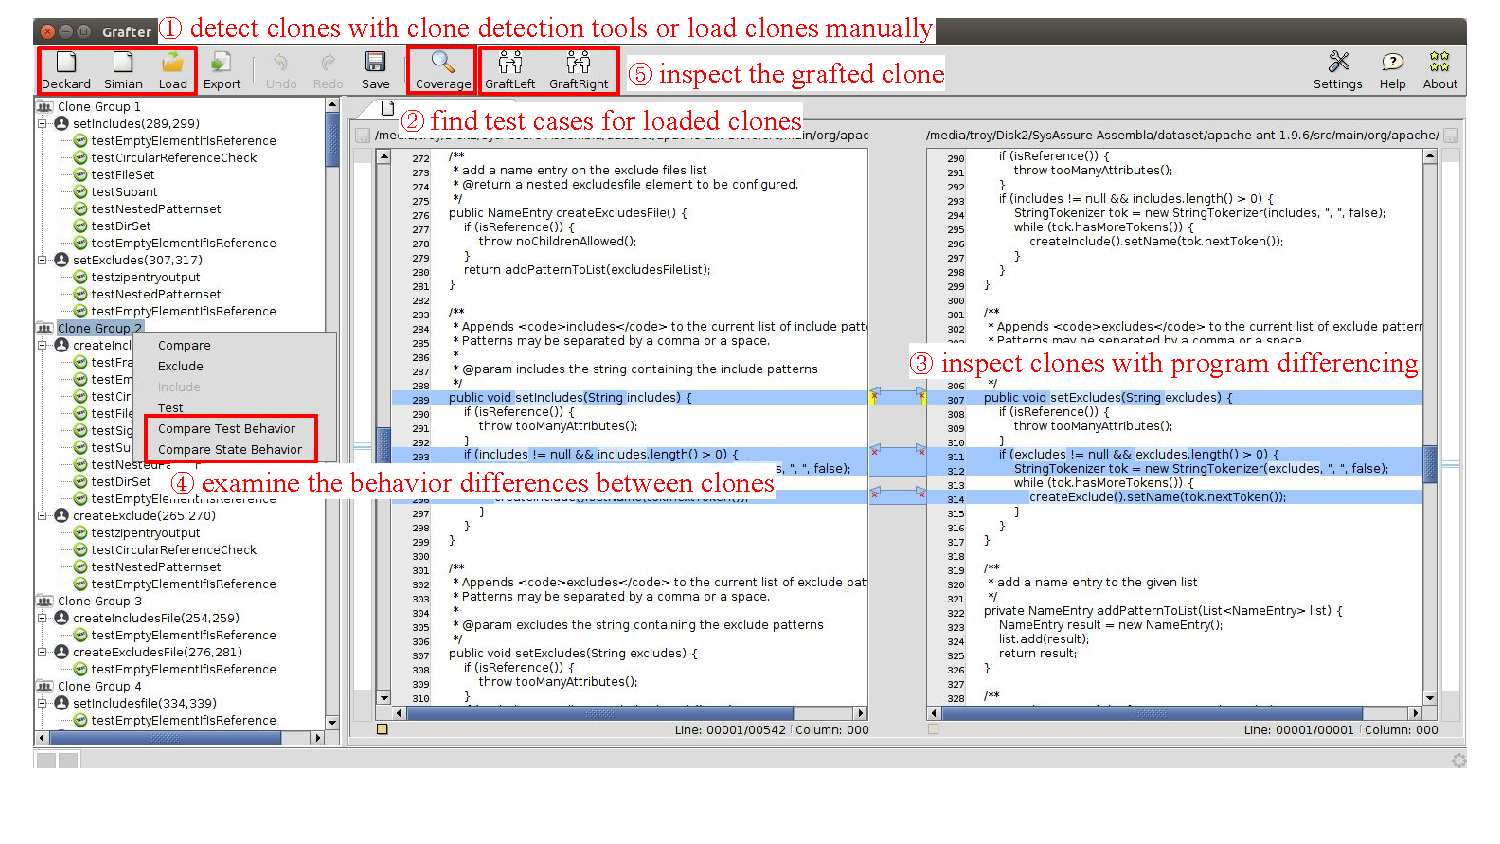
\includegraphics[width=\linewidth]{grafter-screenshot-v3.pdf}
\caption{The screenshot of Grafter}
\label{fig:screenshot}
\end{figure*}

Similar to how organ transplantation may bring incompatibility issues between a donor and its recipient, a grafted clone may not fit the context of the target program due to variations in clone content. For example, if a clone uses variables or calls methods that are not defined in the context of its counterpart, simply copying a clone in place of another will lead to compilation errors. To ensure {\em type safety} during grafting, {\grafter} performs inter-procedural analysis to identify variations in referenced variables and methods. It then adapts the grafted clone using five transplantation rules to handle the variations in referenced variables, types, and method calls. Finally, it synthesizes stub code to propagate input data to the grafted clone and then transfers intermediate outputs back to the recipient. {\grafter} supports differential testing at two levels: test outcomes (i.e., {\it test-level comparison}) and intermediate program states (i.e., {\it state-level comparison}). During differential testing, {\grafter} does not assume that all clones should behave similarly nor considers that all behavioral differences indicate bugs. In fact, a prior study on clone genealogies~\cite{Kim05} indicates that many syntactically similar clones are used in different contexts and have intended behavioral differences. The purpose of differential testing in {\grafter} is rather to illuminate and expose behavioral differences at a fine-grained level {\em automatically} and {\em concretely} by pinpointing which variables' states differ in which test.
 
We evaluate {\grafter} on 52 pairs of nonidentical clones from three open-source projects: Apache Ant, Java-APNS, and Apache XML Security. % To assess {\grafter}'s ability to reuse tests for nonidentical clones, our dataset includes 38 pairs of syntactically identical code fragments except for variations in variables, types, and methods, etc, and 14 pairs are similar code fragments with further variations such as added or deleted statements. 
 {\grafter} successfully grafts and reuses tests in 49 out of 52 pairs of clones without inducing compilation errors. Successfully reusing tests in 94\% of the cases is significant, because currently no techniques enable test reuse for nonidentical clones appearing in the middle of a method. {\grafter} inserts up to 33 lines of stub code (6 on average) to ensure type safety during grafting, indicating that code transplantation and data propagation in {\grafter} are not trivial. To assess its fault detection capability, we systematically seed 361 mutants as artificial faults using the {\major} mutation framework~\cite{just2014major}. We use Jiang et al.'s static cloning bug finder~\cite{Jiang2007} as a baseline for comparison. 
By noticing runtime behavioral discrepancies, {\grafter} is more robust at detecting injected mutants than Jiang et al.\textemdash 31\% more using the test-level comparison and almost 2X more using the state-level comparison. {\grafter}'s state-level comparison also narrows down the number of variables to inspect to three variables on average. Therefore, {\grafter} should complement static cloning bug finders by enabling runtime behavior comparison. Our grafting technology may also have potential to assist code reuse and repair~\cite{weimer2009automatically, Barr2015AST, petke2014using, harman2014babel}. 

% ==================================================
% Motivating Example and Tool Features
% ==================================================
%\section{Motivating Example}
\label{sec:motivation}

This section motivates {\grafter} using an example based on Apache Ant. The change scenario is constructed by us to illustrate the difficulty of catching cloning bugs. Figure~\ref{fig:example} shows the pair of inconsistently edited clones, one from the {\ttt setIncludes} method in the {\ttt Copy} class (lines 6-15 in Figure~\ref{fig:example}a) and the other from the {\ttt setExcludes} method in the {\ttt Delete} class (lines 6-15 in Figure~\ref{fig:example}b). These clones are syntactically similar but not identical---the left program uses a field {\ttt includes} of type {\ttt IncludePatternSet} while the right program uses a field {\ttt excludes} of type {\ttt ExcludePatternSet}. The {\ttt Copy} class implements the task of copying files matching the specified file pattern(s). On the other hand, {\ttt Delete} removes files that do not match the pattern(s). Methods {\ttt setIncludes} and {\ttt setExcludes} both split the input string by a comma and add each pattern to a pattern set, {\ttt includes} and {\ttt excludes} respectively. Figure~\ref{fig:test} shows a test case, {\ttt testCopy}, which creates a {\ttt Copy} object, specifies two copied file patterns as a string {\ttt "src/*.java, test/*.java"}, and then checks if all java files in the {\ttt src} folder and the {\ttt test} folder are copied to a target directory. However, the {\ttt Delete} class is not tested by any existing test. 

%\begin{figure}[!t]
%\centering
%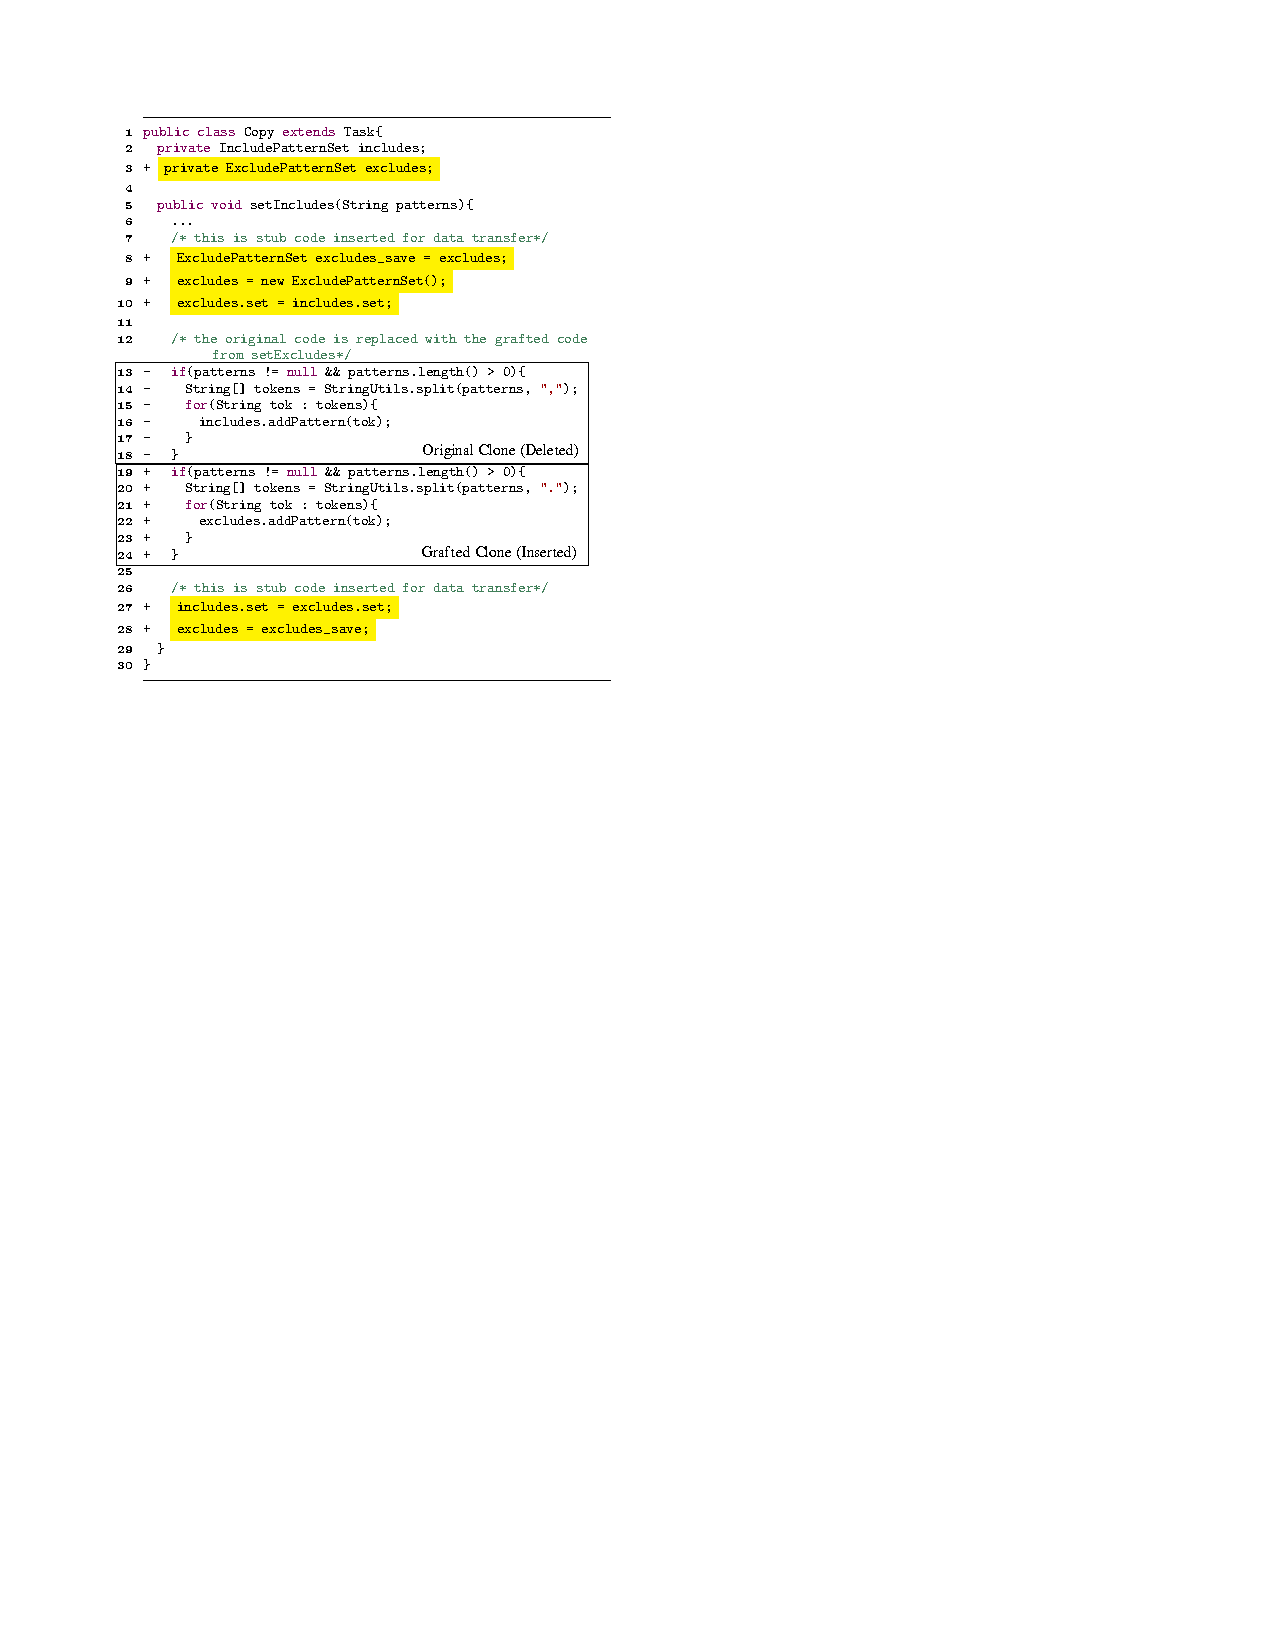
\includegraphics[width=0.45\textwidth]{graftedcode.pdf}
%\caption{{\grafter} grafts the clone in {\ttt Delete} (lines 19-24) in place of the original clone in {\ttt Copy} (lines 13-18) for test reuse. {\grafter} inserts stub code (highlighted in yellow).}
%\label{fig:output}
%\vspace{-4mm}
%\end{figure}

{\ttt StringTokenizer} is a legacy class and its usage is now discouraged in new code. Therefore, Alice updates the use of {\ttt StringTokenizer} API to {\ttt StringUtils.split} in both {\ttt Copy} and {\ttt Delete} in Figure~\ref{fig:example}. However, she accidentally changes the separator from {\ttt `,'} to {\ttt `.'}~in {\ttt Delete} (line 11 in Figure~\ref{fig:example}b). Such mistake is difficult to notice during manual inspection, as these programs are similar but not identical. An existing cloning bug finder by Jiang et al.~would fail to find the mistake, as it checks for only three pre-defined cloning bug types via static analysis~\cite{Jiang2007}: renaming mistakes, control construct inconsistency, and conditional predicate inconsistency. Accidentally replacing the separator does not belong to any of the pre-defined cloning bug types.

{\bf Inspect clones.} Alice can inspect clones by right clicking a clone group and select ``Compare''. Each clone in the group is named in the format of ``(start line number, end line number)'' by default. Alice can double-click and rename a clone, but it has to be in the format of ``XYZ(start line number, end line number)''. Grafter automatically excludes trivial clone groups (e.g., clones in test files) and mark them in red. If Alice believes Grafter mistakenly filters out a clone group, Alice can re-add this group by right-clicking on it and select "Include". When inspecting clones, you can discard a clone group by right-click -> Exclude. Alice can click ``Export'' and save all clone groups of interest to an xml file. All excluded clones will be discarded and not exported to the xml file.

{\bf Find test cases for clones.} Alice does not need to specify the test cases. Instead, Alice can just click the ``Coverage'' button and {\grafter} will automatically locate test cases for each clone. This is very helpful when Alice is investigating a large code base with a large number of test cases.

{\bf Reuse test and examine behavior differences.} {\grafter} supports the behavior comparison in two granularities. Alice can compare the test outcomes of two clones by right-clicking the clone group and selecting ``Compare Test Behavior''. The comparison results are represented in a table and behavioral differences are highlighted in red for ease of investigation. The first column shows names of test cases. The second and third columns show whether each clone passes or fails the corresponding test case. The last column shows the comparison result. Green means both clones are consistent on this test and red means their test outcomes are different.

Alice can also compare the intermediate state values of two clones by right-clicking the clone group and selecting ``Compare State Behavior''. In the state-level comparison table, the first and third columns show the name of corresponding variables referenced by code clones, and the second and fourth columns show the values of variables in the format of XML. Grafter prints the value of an object in XML using XStream.

To reuse the same test {\ttt testCopy} for {\ttt Delete}, {\grafter} grafts the clone from {\ttt Delete} in place of the original clone in {\ttt Copy}, as shown in Figure~\ref{fig:output}. As the grafted code uses an undefined variable {\ttt excludes}, {\grafter} also ports its declaration to {\ttt Copy.java}. {\grafter} ensures that the grafted clone receives the same input data by populating {\ttt excludes} with the value of {\ttt includes} (lines 8-10) and transfers the value of {\ttt excludes} back to {\ttt includes} (lines 27-28). Therefore, the value of {\ttt excludes} can flow into the same assertion check of the original test. Additional stub code generated by {\grafter} is highlighted in yellow in Figure~\ref{fig:output}.

After grafting, {\grafter} runs {\ttt testCopy} on both clones and finds that the test now fails on {\ttt Delete}, because the string is not split properly. To help Alice further diagnose failure symptoms, {\grafter} shows that {\ttt tokens} has a list \{ {\ttt "src/*.java"}, {\ttt "test/*.java"}\} in {\ttt Copy} but \{ {\ttt "src/*"}, {\ttt "java, test/*"}, {\ttt "java"} \} in {\ttt Delete} due to a wrong split. {\grafter} also shows that this difference has propagated to corresponding variables {\ttt includes} and {\ttt excludes}.

% ==================================================
% Implementation
% ==================================================
\section{Grafter Implementation}
{\grafter} takes a pair of clones and an existing test suite as input and constrasts the runtime behavior of the clones. The core of {\grafter} is to transplant test cases between clones so that {\grafter} can exercise clones with the same test. This section briefly discusses the transplantation process of {\grafter}. The details are described in our previous work~\cite{zhang2017automated}.

\noindent{\bf Variation identification.} {\grafter} first perform inter-procedural analysis to identify the input and output parameters referenced by each clone and its subroutines to expose its de-facto testing interface. {\grafter} then matches the input and output parameters between clones and detect the paramaters that are defined in one clone but not in the counterpart clone.

\noindent{\bf Code transplantation.} Simply copying and pasting a clone in place of its counterpart clone could lead to compilation errors due to variations in clone content. {\grafter} applies five transplantation
rules to ensure type safety during code transplantation.  

\noindent{\bf Data propagation.} Similar to how surgeons reattach blood vessels to ensure the
blood in the recipient flows correctly to the vessels of the transplanted organ, {\grafter} also needs to make sure the input data flows correctly into the grafted clone and the updated values flows back to the same assertion check of the original test. Therefore, {\grafter} applies four heuristics to insert stub code to
ensure that (1) newly declared variables consume the same input data as their counterparts in the recipient and (2) the updated values flow back to the same test oracle.

\noindent{\bf Differential testing.} {\grafter} supports behavior comparison at two levels. The test-level comparison runs the same test on two clones and compares the test outcomes. If a test succeeds on one clone but fails on the other, behavior divergence is noted. The state-level comparison compares the intermediate program states for affected variables at the exit(s) of the clones. {\grafter} instruments code clones to capture the updated program states at the exit(s) of clones. {\grafter} uses the XStream library\footnote{\url{http://x-stream.github.io/}} to serialize the program states of affected variables in an XML format. Then it checks if two clones update corresponding variables with the same values.

{\grafter} is built on top of an open-source visual diff and merge tool, JMeld.\footnote{\url{https://github.com/albfan/jmeld}} Configure {\grafter} and run it using the following command. The user configuration file asks the user to speficy the source and test folders in a project as well as the build system in the command so that {\grafter} can perform the test coverage analysis.

\begin{lstlisting}
$ java -jar grafter.jar /path/to/your/config/file
\end{lstlisting}

% ==================================================
% Step-by-step Demonstration
% ==================================================
\section{Step-by-step Demonstration}
\label{sec:demo}

\begin{figure}[!t]
\centering
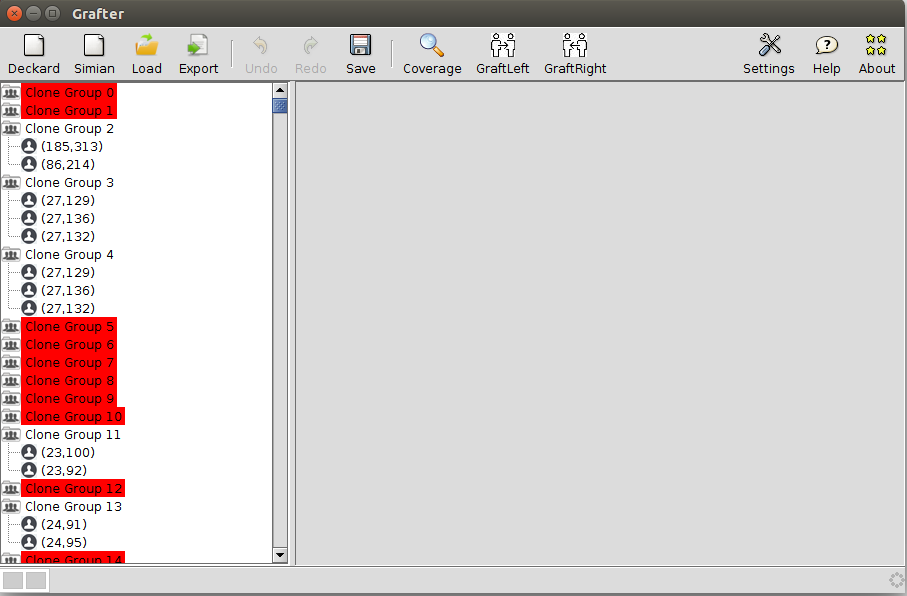
\includegraphics[width=0.5\textwidth]{grafter_new.png}
\caption{Load detected clones and proactively filter out low-quality clones.}
\label{fig:load}
\end{figure}

\subsection{Detect and Load Clones to Grafter}

To ease the effort of detecting clones in a large code base, {\grafter} integrates two clone detection tools, Deckard~\cite{Jiang2007a} and Simian~\cite{simian} (see \ding{172} in Figure~\ref{fig:screenshot}). Deckard parses source code to abstract syntax trees (ASTs) and detects similar code via tree comparison, while Simian is a commercial tool that detects duplicated code via text comparison. Users can also specify the clones of interest in an xml file and load these clones manually by clicking the ``Load'' button.

As noted by previous studies~\cite{bellon2007comparison, roy2009comparison}, clone detection tools may emit a large amount of plausible clones---clones that are syntactically similar but are trivial to analyze. {\grafter} proactively detects such trivial clones using several simple heuristics and marks them in red, as shown in Figure~\ref{fig:load}. {\grafter} considers a group of clones is trivial if (1) clones are in comments or declaration statements, (2) clones are not syntactically complete, or (3) clones are from the same method. {\grafter} also marks clones in test files in red, since {\grafter} aims to contrast the runtime behavior of clones in functional code.

\subsection{Inspect Clones}

Users can inspect the textual differences of loaded clones by right clicking a clone group and select ``Compare'' (see \ding{174} in Figure~\ref{fig:screenshot}). We customized the existing program differencing feature in JMeld to only compute the differences between the cloning regions in two Java files. So users only need to focus on the textual differences between the cloning regions, instead of the entire files. Each clone in the group is named in the format of ``(start line number, end line number)'' by default. Users can update the cloning region or rename it with the method name by double clicking the clone label.

During the manual inspection, if a user considers a clone group to be trivial, she can filter out the clone group by right clicking the group label and select ``Exclude.'' Similary, if a user finds a clone group is mistakenly excluded, she can re-add the group again by right clicking the group label and select ``Include.''

\begin{figure}[!t]
\centering
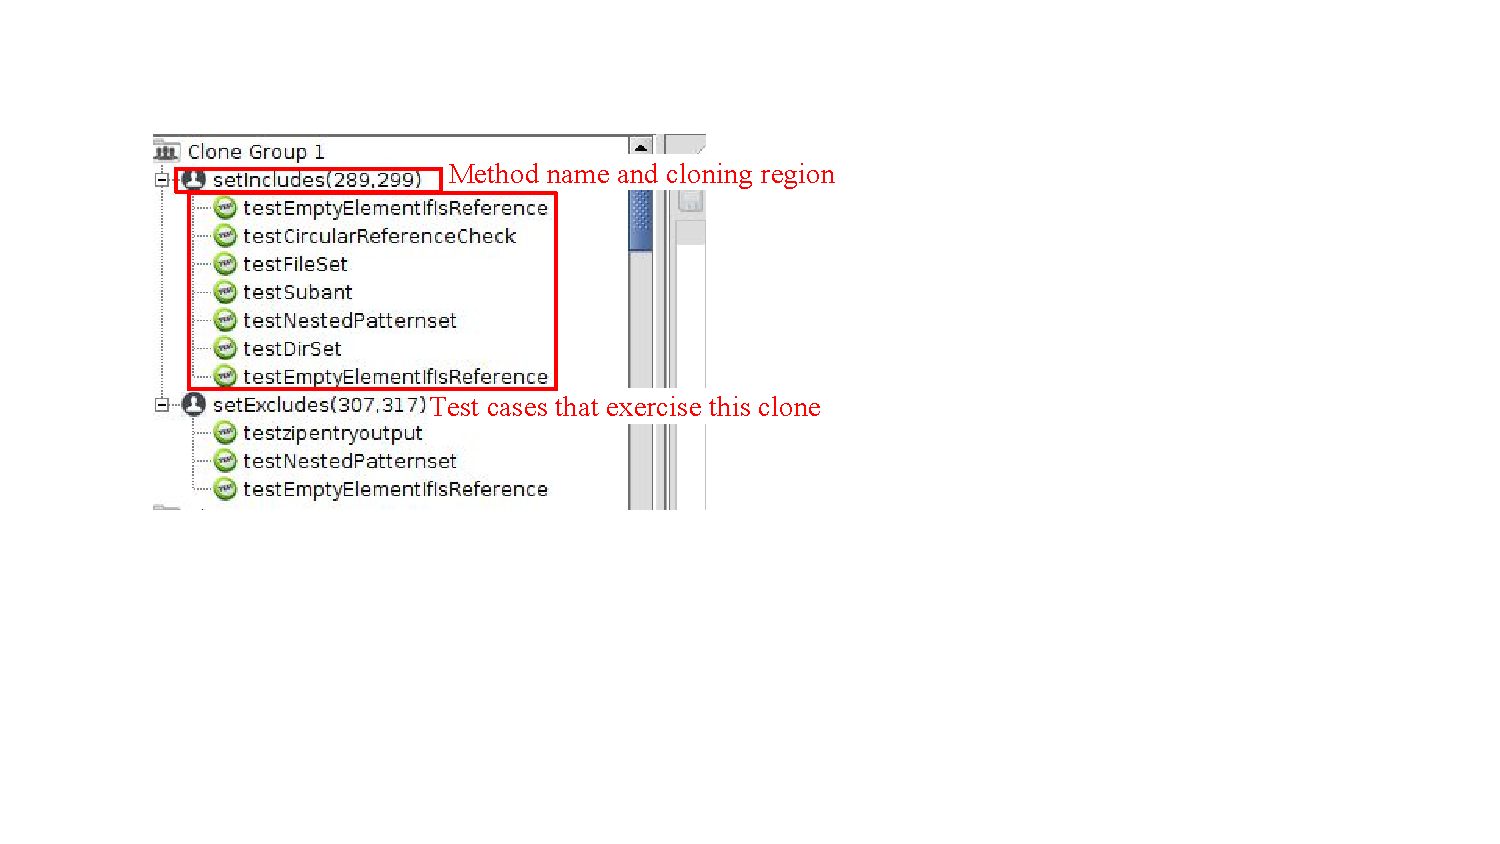
\includegraphics[width=0.45\textwidth]{clone-group-view.pdf}
\caption{The clone group view.}
\label{fig:output}
\end{figure}

\subsection{Find Test Cases of Clones}

When a target project contains a large number of clones and test files, it may not be easy to manually find the test cases for each detected clone. Instead, a user can click the ``Coverage'' button and {\grafter} will automatically locate test cases for each loaded clone (see \ding{173} in Figure~\ref{fig:screenshot}). To analyze the test coverage of code clones, {\grafter} instruments each clone to print out their call stack traces and gathered the test cases appearing in the traces. Note that {\grafter} requires at least one clone in the clone group to be executed by one or more tests in order to reuse tests on its counterpart clones. If none of the clones in a group is covered by a test case, a user should discard the clone group by right clicking and select ``Exclude.''

\subsection{Reuse Tests and Examine Behavioral Differences}

\begin{figure}[!t]
\centering
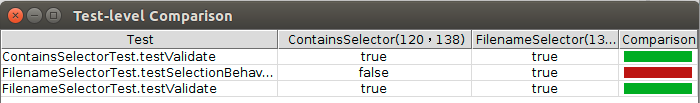
\includegraphics[width=0.5\textwidth]{grafter-test-diff.png}
\caption{The test-level behavior differencing of Grafter}
\label{fig:test}
\end{figure}

\begin{figure}[!t]
\centering
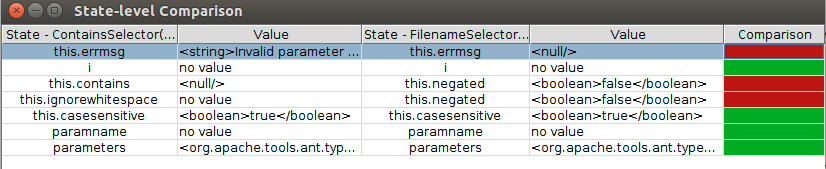
\includegraphics[width=0.5\textwidth]{grafter-state-diff.png}
\caption{The state-level behavior differencing of Grafter}
\label{fig:state}
\end{figure}

\noindent{\bf Test-level Comparison.} Users can compare test outcomes of two clones by right clicking the clone group and selecting ``Compare Test Behavior''. The comparison results are represented in a table and behavioral differences are highlighted in red for ease of investigation, as shown in Figure~\ref{fig:test}. The first column shows names of test cases. The second and third columns show whether each clone passes or fails the corresponding test case. The last column shows the comparison result. Green means both clones are consistent on this test and red means their test outcomes are different.

\noindent{\bf State-level Comparison.} Users can compare intermediate state values of two clones by right clicking the clone group and selecting ``Compare State Behavior''. In the state-level comparison table in Figure~\ref{fig:state}, the first and third columns show the name of corresponding variables referenced by code clones, and the second and fourth columns show the values of variables in the format of XML. {\grafter} prints the value of an object in XML using XStream. Users can view the complete xml representation of an object by hovering the mouse over the corresponding cell, as shown in Figure~\ref{fig:hover}.

\begin{figure}[!t]
\centering
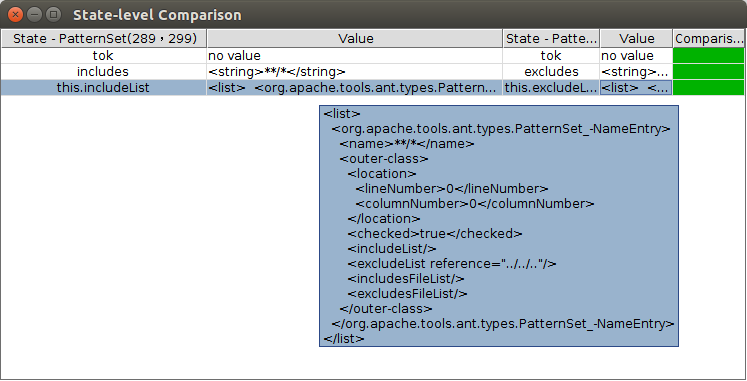
\includegraphics[width=0.45\textwidth]{hover.png}
\caption{Inspect the intermediate state value.}
\label{fig:hover}
\end{figure}

\subsection{Inspecting Grafted Clone} 

Note that the inserted stub code doesn't persist during test transplantation and therefore doesn't need to be comprehended by the developers. Yet {\grafter}'s GUI still allows users to experiment with clone grafting and inspect the intermediate grafted code. Users can graft the left clone to replace the right one and view the grafted code in the diff view by clicking ``Graft Left'' in the top menu bar (vice versa). Users can further test the grafted code by right clicking the clone group and select ``Test''. Users can undo and redo the previous graft by clicking the "Undo" and "Redo" buttons on the top menu bar respectively.

\begin{figure}[!t]
\centering
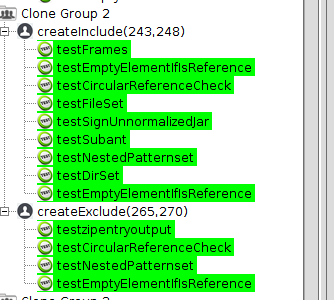
\includegraphics[width=0.4\textwidth]{test-grafted-clone.png}
\caption{Test the grafted clone.}
\label{fig:hover}
\end{figure}

% ==================================================
% Related Work
% ==================================================
\section{Related Work} 
The most related test reuse technique is Skipper. Skipper copies associated portions of a test suite when developers reuse code~\cite{2013:spe:makady}. It determines relevant test cases and transforms them to fit the target system. Skipper is built on Gilligan~\cite{holmes2007supporting, 2012:tosem:holmes} and requires users to provide a {\em pragmatic reuse plan} to establish the mapping of reused entities (e.g., classes, methods) from the original system to the target system. Skipper assumes that clones are full-feature clones at the level of methods and classes. This requirement makes it difficult to apply Skipper to sub-method level clones found by existing clone detectors. It is infeasible to empirically compare {\grafter} with Skipper due to the requirement of having a reuse plan. %\textemdash rename reused entities as needed, replace references to non-reused entities with {\em holes}, fill in these holes with stub code that mocks the objects and method calls by recording and replaying the execution traces from the original program. 
When the reuse plan is incomplete, the resulting tests produced by Skipper could contain compilation errors and developers must fix them manually.

{\grafter} differs from Skipper in three perspectives. First, {\grafter} supports sub-method level clones without explicit interfaces. Second, {\grafter} does not require a reuse plan but rather leverages the syntactic resemblance between clones to guide the grafting process. Third, Skipper may require manual adjustments to fix compilation errors when the reuse plan is incomplete. In contrast, {\grafter} is fully automated using transplantation rules and data propagation heuristics.

% ==================================================
% Summary
% ==================================================
\section{Summary}
\label{sec:summary}
Up to a quarter of software systems consist of code clones from somewhere else. However, the cost of developing test cases is high, which makes test reuse among similar code attractive. This paper introduces {\grafter}, the first test transplantation and reuse approach for enabling runtime behavior comparison between clones. To handle the use of different types, methods, and variables in clones, {\grafter} automatically inserts stub code to propagate data between corresponding variables while ensuring type safety. {\grafter}'s code transplantation succeeds in 94\% of the cases, and its fine-grained differential testing can detect more seeded faults than a baseline static cloning bug finder. This result shows {\grafter}'s potential to assist developers in catching subtle bugs during copy and paste and to aid developers in comprehending the runtime behavior of nonidentical clones. 

%\section{Acknowledgement} 

\balance
\bibliographystyle{ACM-Reference-Format}
\bibliography{grafter}
\end{document}
